\section{Design}

\begin{comment}
\subsection{Components}
Overview of whole system and functionalities of each component. 

\subsection{Interfaces}
Introduce forwarding table (between data plane and control plane), hint (within control plane between controller and nodes), NIB (between discovery modules and control plane)

\subsection{Flexible Data plane}
Our data plane can be based on existing proxy servers (e.g., Apache server) used by production networks. What flexibility we need from data plane.
\begin{itemize}
	\item Understand and execute based on the forwarding table.
	\item Provide information for in-band passive measurement.
\end{itemize}

\subsection{Discovery}
Discovery consists of local process running on each node to output local NIB, and global process that combines the local NIBs to output a global NIB.

\begin{itemize}
	\item how to compute global NIB from local NIBs
	\item when to inform global control process of a change in global NIB to prevent frequent recalculating (when it is converged?) \jc{need some idea...}
\end{itemize}

\subsection{Control plane}
The control plane design has three parts: global control process, local control process, and merging algorithm.

Global control process: globally coordinated resource share. output global hint based on application-level goals. Coarse time granular.

Local control process: detect connection failure/congestion from local NIB and output local hint.

Merging algorithm: merge global hint from multiple controllers and local hint. need to meet requirements: (i) correctness, and (ii) prefer local hint when local hint strongly suggests current forwarding table is hopeless.
\end{comment}


\begin{figure*}[t]
\centering
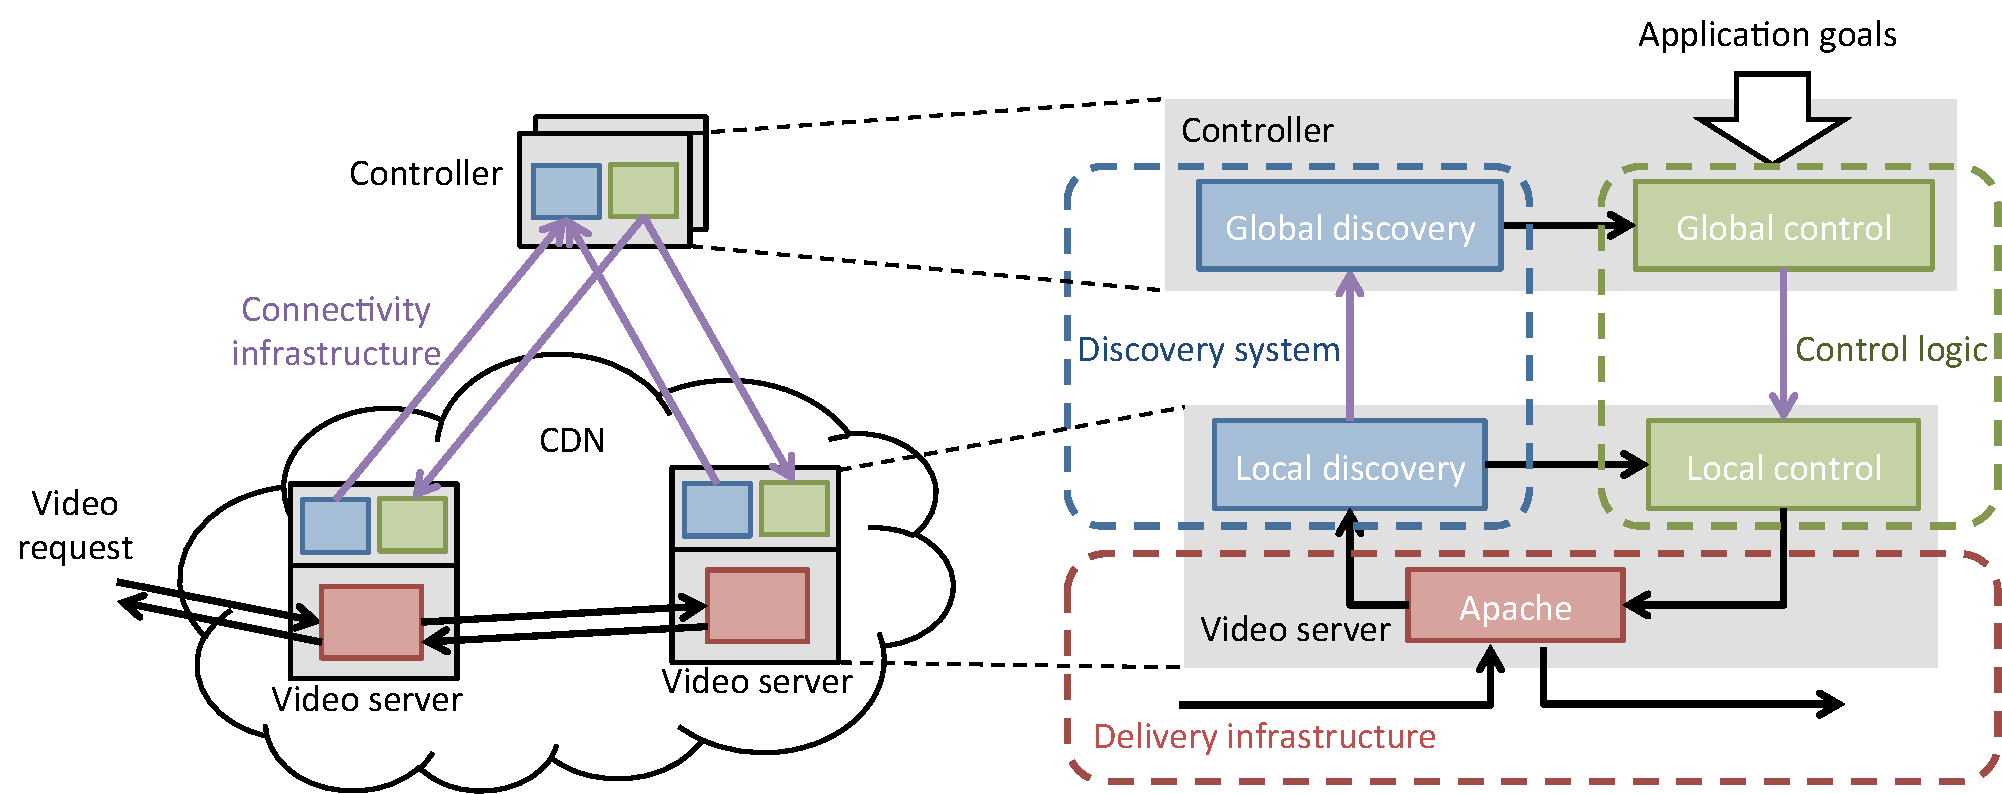
\includegraphics[width=2.0\columnwidth]{figures/system-overview-2.pdf}
\caption{System overview of SDCDN.}
\label{fig:system-overview}
\end{figure*}

This section first gives an overview of the components of a software-defined CDN (\SDCDN) and then presents the design choices and implementation of each components. 

\subsection{Overview of \SDCDN}

There are five components in  (see Figure~\ref{fig:system-overview}). 

\myparatight{\Data} This includes servers as well as any other network elements (such as cache) that perform content delivery and support an interface to measure and control the forwarding state. For simplicity, we call such nodes servers in \data. In live video streaming, the \data consists of several video origin server and a set of intermediate and edge servers that forward the content request to the origin server or a cached replica and deliver the requested content back.

\myparatight{\Dissemination} This communication between servers and the centralized controller transits the \dissemination. It must support bidirectional communication -- collecting statistics from servers to the controllers and disseminating decisions from the controllers to servers, and optionally support specific protocols to enforce receiving order of messages.

\myparatight{\Discovery} The \discovery runs both on servers and controllers. Local process of \discovery running on each server gathers statistics on both network states (e.g., link failure) and application information (e.g., which streams are more popular) through the measurement interface provided by \data. It then sends the summarized result to \localControl (as discribed below for real-time adaptation) and the controller through \dissemination. The global process of \discovery in the controller collects the network states and application information, and generates a network information base (NIB) and stream information base (SIB) respectively.

\myparatight{\GlobalControl} \GlobalControl performs joint optimization to coordinate network resource and video streams based on NIB and SIB generated by \discovery. The result of \globalControl is in form of a hint to each server that specifies for the request of each stream a set of next hop servers. The \globalControl has customized logic to support application-level goals (e.g., video quality optimization).

\myparatight{\LocalControl} \LocalControl receives hints from multiple controllers and measurement from local process of \discovery, and performs real-time control on the behavior of \data. 



\subsection{\Data}

The \data consists of video servers that perform content delivery for a wide range of protocols. We use HTTP as the basic transport protocol. Although traditional belief is that UDP or other propriatory protocols are better than HTTP because they reduce the latency, streaming live video over HTTP has recently been developed and advocated by industry in various protocols (e.g., \cite{HLS, HDS}) and standards \cite{dash}. The driven force of this trend is that HTTP has better middlebox support than other protocols and is well supported by CDNs to delivery web contents.

\mypara{Support multi-bitrate chunk-based live streaming with standard web servers}

\mypara{Forwarding table} map between a stream prefix and a forwarding strategy (forward the request to next hops by specified probability distribution and specified timeout). introduce format: stream prefix, set of next hops, timeout

\begin{figure}[h]
\centering
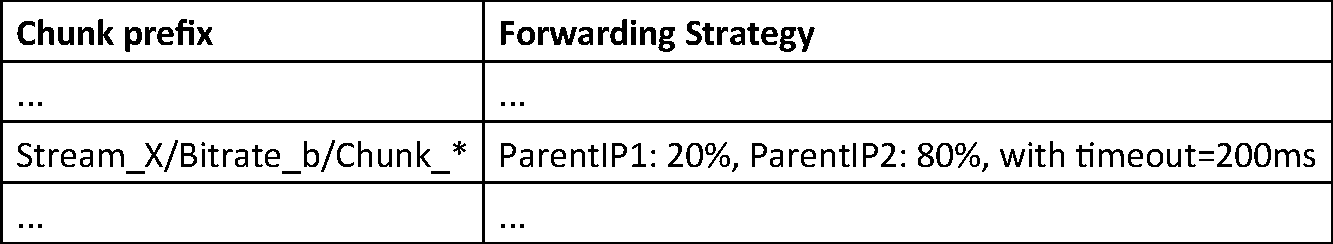
\includegraphics[width=1.0\columnwidth]{figures/forwarding-table-format.pdf}
\caption{Forwarding table}
\label{fig:forwarding-table}
\end{figure}

\mypara{Control interface} 
\begin{itemize}
	\item Implement forwarding table
	\item For a time-out request, change to another destination.
\end{itemize}

\mypara{Measurement interface}
\begin{itemize}
	\item Request received
	\item Request time-out
	\item Request download time, downloaded size
	\item Request for unknown request
	\item Request from unexpected interface
\end{itemize}

\mypara{Integration with standard HTTP web server} 
\begin{itemize}
	\item What Apache already provides (request count, loop detection, cache, timeout, multi-path): why is future-proof
	\item Integration issues
\end{itemize}



\subsection{\Dissemination}

The \dissemination maintains the communication between controller and servers. It is used by both \discovery and \decision. 

\begin{itemize}
	\item Design choices: in-band vs. out-band, point-to-point vs. multicast protocol. Our implementation uses RPyC: out-band and point-to-point (why)
	\item Deal with connection failure. Notify sender after timeout
	\item Traffic aggregation at egress/ingress of cluster. 
\end{itemize}


\subsection{\Discovery}

The goal of \discovery is to maintain a global on network states and stream states based on the information collected from measurement interface of \data. Network states include the network topology, performance of links within and between clusters of video servers.  Stream states include statistics of each video stream  (e.g., number of requests). We use two data structures, network information base (NIB for shor) and stream information base (SIB for short) to store the network states and stream states separately.

The basic entity of network state can be the pysical links or overlay links between two servers depending on the visibility of the measurement method. In this work, we use passive in-band measurement that measures throughput of video delivery between two servers, and thus the network state consists of throughput of all used overlay link.  Active measurement is also viable through cooperation between local monitoring processes running on different servers, and can discover more information, for example, physical link topology (via traceroute). However, these are out of our scope. \jc{Where to get topology information?}

A local monitoring process in each server collects local measurement results from measurement interface of \data and generates local NIB and SIB. Both need to be with timestamps. 

The local NIB and SIB will be sent back via \dissemination to the global monitoring process in controller periodically. These local NIBs and SIBs will be merged to update the global NIB and SIB.

The NIB and SIB are used to activate \decision when a significant change is detected in NIB or SIB. In real-time, if local SIB indicates a chunk request has timed out, the \localControl will be immediately activited and perform real-time reaction (for example, redirect the request to another neighbor). The global NIB and SIB are updated in a coarser time scale. When one or more links depart too much from its previous performance, it will initiate the \globalControl.

New stream establishment is also done by \discovery.

Finally, the traffic initiated by \discovery scales with more servers and more frequent, which places heavy burden on both \dissemination and \decision. Several widely used technique in SDN can be leveraged cluster-based traffic aggregation~\cite{?} and incremental update~\cite{?} to improve scalability.



\subsection{\Decision}

The \decision runs in both the controllers and servers, and makes decisions in three time scales.

\myparatight{Global coordination} The \globalControl in controllers is activated by global NIB and SIB generated by \discovery, makes decision of the forwarding strategy on each server for each stream, and sends the decision to each server by \dissemination. Such global decision is a soft control called global {\it hint}, based on which the \localControl decides forwarding table in real-time. \jc{Format of hint}

\myparatight{Realtime coordination} \localControl makes realtime coordination using two separate logics -- the {\it local decision algorithm} and the {\it merging algorithm}. The local decision algorithm gets triggered by local NIB and SIB and generates a local hint. On receiving any of local hint or global hint from one controller, the merging algorithm merges the newest version of local and global hints to update forwarding table in \data.

\myparatight{Application goals} The \decision also provides the flexibility in changing its logics to meet various application level goals. For example, the \decision can be configured to optimize for video quality (weighted sum of satisified bitrate) or bandwidth cost per cluster. In doing so, we must support runtime modification to the logics in both \globalControl and \localControl (local decision and merging algorithm). One possible approach is to write these logics in scripts which are called by another process that support runtime replacement of these scripts.









